% --------------------------------------------------------------------------------------------
% 										Capitulo 4
% --------------------------------------------------------------------------------------------

\chapter{Descrição da Pipeline}

Este capítulo descreve detalhadamente a pipeline de simulação desenvolvida, incluindo decisões de design, arquitetura do software, casos de uso e exemplos de utilização

\section{Decisões de Design}

Nesta seção, discutimos as principais decisões de design tomadas durante o desenvolvimento da pipeline, incluindo a escolha de tecnologias, padrões de arquitetura e estratégias de implementação.

\subsection{Princípios Orientadores}

O desenvolvimento da pipeline de simulação foi conduzido a partir de um conjunto de princípios de engenharia de software definidos para atender às necessidades específicas do processamento de dados observacionais em radioastronomia. Simulações desse tipo frequentemente envolvem múltiplos modelos físicos, diferentes configurações instrumentais e grandes volumes de dados, exigindo uma arquitetura capaz de acomodar modificações e expansões ao longo do ciclo de desenvolvimento \cite{sharma2025karabo}.

A modularidade foi adotada como princípio central da implementação. Nessa abordagem, cada etapa do fluxo de processamento é encapsulada em componentes independentes responsáveis por tarefas específicas, como geração de mapas de entrada, simulação instrumental, produção de Time Ordered Data e reconstrução de mapas. Essa organização reduz o acoplamento entre diferentes partes do sistema e favorece a reutilização de componentes em distintos cenários de simulação  \cite{martin2008cleancode}.

A extensibilidade constituiu outro requisito fundamental. Em aplicações voltadas à radioastronomia observacional, é comum a necessidade de incorporar novos modelos de ruído, estratégias de varredura, descrições instrumentais ou métodos de reconstrução. Dessa forma, a arquitetura foi concebida para permitir a inclusão de novas funcionalidades com impacto mínimo sobre os módulos já existentes, preservando a consistência do sistema e reduzindo o custo de manutenção.

A testabilidade foi igualmente priorizada. A separação funcional entre os módulos permite que cada componente seja validado individualmente por meio de testes específicos, facilitando a identificação de inconsistências e contribuindo para a confiabilidade dos resultados produzidos pela pipeline. o que é especialmente importante em simulações científicas, onde a precisão e a robustez dos resultados são cruciais para a interpretação dos dados observacionais.

O processo de observação simuladas geralmente envolve conjuntos de dados de grandes dimensões, principalmente em longos periodos de observação. Por essa razão, a implementação buscou minimizar operações redundantes, otimizar o fluxo de dados entre os módulos e explorar estruturas computacionais adequadas para processamento em larga escala.

Por fim, buscou-se garantir um elevado nível de documentação do software. Além da utilização de convenções padronizadas de nomenclatura, foram adotadas práticas de documentação diretamente associadas aos módulos implementados, descrevendo suas funcionalidades, parâmetros de entrada e formatos de saída. Essa abordagem facilita tanto a reprodução dos experimentos quanto a utilização futura da pipeline por outros pesquisadores.

\subsection{Escolhas Tecnológicas}

A implementação da pipeline foi realizada utilizando a linguagem Python, adotando como requisito mínimo a versão 3.10. Essa escolha foi motivada pela ampla utilização da linguagem em computação científica, pois a ligunagem Python  oferece uma sintaxe clara e concisa, o que contribui para a legibilidade do código e facilita a colaboração entre pesquisadores de diferentes áreas. Além disso, a comunidade científica tem desenvolvido uma vasta gama de bibliotecas e ferramentas em Python, como NumPy, SciPy, Astropy e Healpy, que são amplamente utilizadas para processamento de dados astronômicos e análise de mapas celestes.

Entre as bibliotecas utilizadas, destacam-se:

\begin{itemize}
    \item \textbf{NumPy:} Recorreu-se como base para manipulação de arrays, operações numéricas e manipulação de eficiénte de estrutura de dados multidimensionais. Sua implementação Sua implementação otimizada para operações vetorizadas permite realizar cálculos envolvendo grandes volumes de dados com desempenho significativamente satisfatório e superior a abordagens baseadas em loops tradicionais \cite{harris2020array}.
    \item \textbf{SciPy:} Adotado para complementar as funcionalidades do NumPy, fornecendo uma ampla gama de algoritmos e rotinas para processamento de dados, otimização, integração, interpolação e processamento de sinais. A biblioteca SciPy é amplamente reconhecida por sua eficiência e confiabilidade em aplicações científicas, o que a torna uma escolha natural para a implementação de algoritmos de simulação e análise de dados em radioastronomia \cite{virtanen2020scipy}.
    \item \textbf{Astropy:} Utilizada para manipulação de coordenadas celestes, conversão de unidades, sistemas temporais e outras operações relacionadas à astronomia. A biblioteca Astropy é amplamente adotada na comunidade astronômica devido à sua robustez, flexibilidade e ampla gama de funcionalidades específicas para o processamento de dados astronômicos \cite{Astropy2022}.
    \item \textbf{Healpy} Empregada para manipulação de mapas celestes em formato HEALPix, que é um formato amplamente utilizado para representar dados astronômicos em uma esfera. A biblioteca Healpy oferece uma série de funções para criar, manipular e visualizar mapas HEALPix, facilitando a implementação de algoritmos de simulação e análise de dados em radioastronomia \cite{gorski2005healpix}.
    \item \textbf{Matplotlib:} Aplicou-se essa biblioteca para visualização de dados e resultados, permitindo a criação de gráficos, mapas e outras representações visuais dos dados simulados. A biblioteca Matplotlib é amplamente utilizada na comunidade científica para visualização de dados em Python, oferecendo uma ampla gama de opções de personalização e suporte para diferentes tipos de gráficos \cite{hunter2007matplotlib}.
\end{itemize}

Em conjunto, essas tecnologias fornecem a infraestrutura computacional necessária para a implementação dos diferentes módulos da pipeline, atendendo simultaneamente aos requisitos de desempenho, extensibilidade e reprodutibilidade definidos na seção anterior.


\subsection{Paradigmas de Programação}

A estruturação da pipeline foi conduzida utilizando conceitos de Programação Orientada a Objetos (POO), combinados com princípios de \textit{Domain-Driven Design} (DDD) e padrões de projeto amplamente empregados em engenharia de software. Essa combinação permitiu estruturar o código de forma alinhada aos requisitos científicos do problema, favorecendo a organização dos componentes, a reutilização de funcionalidades e a evolução da arquitetura ao longo do desenvolvimento.

A POO foi adotada como paradigma principal para o desenvolvimento dos módulos da pipeline, permitindo a definição de classes e objetos que encapsulam dados e comportamentos relacionados a diferentes aspectos do processo de simulação \cite{gamma1994designpatterns}. Essa abordagem facilita a modelagem de entidades complexas, como instrumentos de observação, estratégias de varredura, de ruído, etapas de processamento e algoritmos de reconstrução, permitindo que cada elemento seja tratado como uma unidade independente e bem definida dentro do sistema.

Além da organização estrutural proporcionada pela POO, foram incorporados conceitos de \textit{Domain-Driven Design} (DDD). Essa abordagem promove uma organização que reflete a realidade científica do problema. Essa abordagem favorece a clareza e a expressividade do código, facilitando a comunicação entre os desenvolvedores e os especialistas na área, além de contribuir para a manutenção e evolução da pipeline ao longo do tempo \cite{evans2003ddd}. Como resultado, os módulos da pipeline foram organizados em torno de conceitos pertencentes ao domínio da radioastronomia observacional, favorecendo a clareza da arquitetura e simplificando a manutenção do código.

Para aumentar a flexibilidade do sistema, foram empregados padrões de projeto específicos em situações recorrentes da implementação. por exemplo, o padrão \textit{Strategy} foi utilizado para encapsular diferentes algoritmos de reconstrução, permitindo que a escolha do método seja feita de forma dinâmica durante a execução da pipeline . O padrão \textit{Factory} foi adotado para criar instâncias de diferentes tipos de instrumentos ou estratégias de varredura, facilitando a extensão do sistema com novos modelos sem a necessidade de modificar o código existente. Por sua vez, o padrão \textit{Observer} foi empregado em situações que exigem comunicação entre componentes desacoplados, permitindo que modificações de estado em determinados módulos sejam automaticamente propagadas para elementos dependentes \cite{gamma1994designpatterns}.

Em conjunto, esses paradigmas e padrões de projeto fornecem a base arquitetural que sustenta a implementação da pipeline, permitindo que sua estrutura permaneça compatível com os requisitos de extensibilidade, manutenção e evolução científica estabelecidos para o projeto.

\section{Modelagem \label{sec.modelagem}}
  


\subsection{Diagrama de Classes Geral}

A arquitetura da pipeline foi modelada utilizando os princípios da Programação Orientada a Objetos, permitindo representar os diferentes elementos do processo observacional por meio de entidades computacionais bem definidas. Essa abordagem favorece a separação de responsabilidades entre os componentes do sistema e facilita a expansão da pipeline para novos cenários de simulação.

\begin{figure}[hbtp]
    \centering
    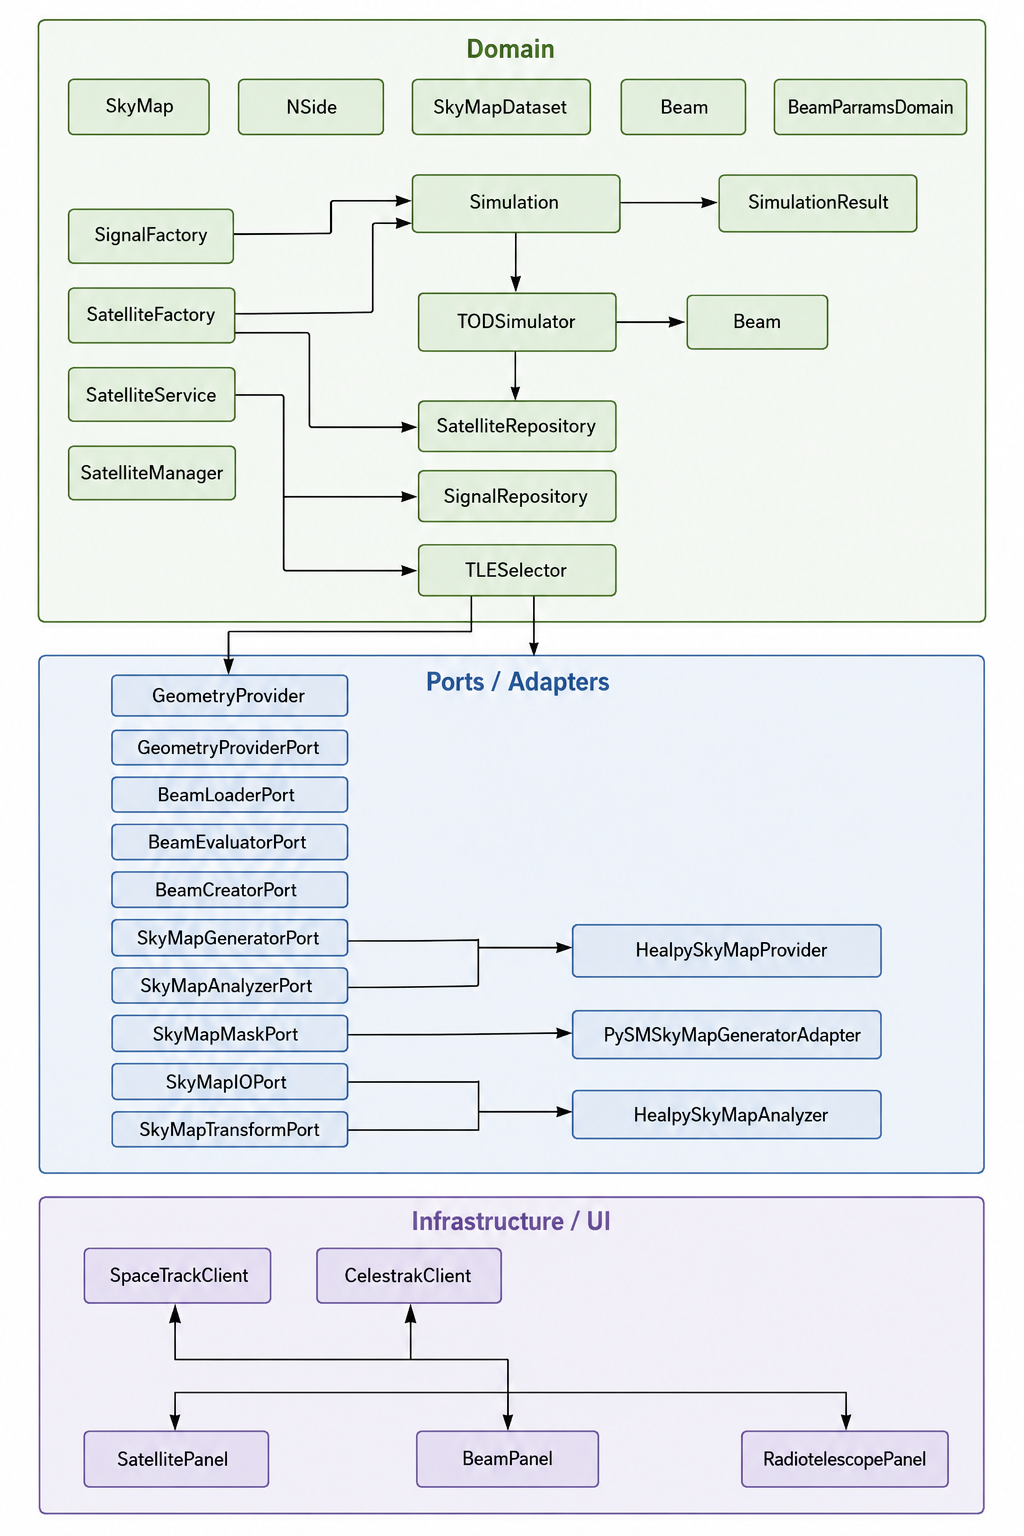
\includegraphics[scale=.4]{Figuras/diagrama_classe_pipeline0.png}
    \caption{Diagrama de classes geral da pipeline de simulação. Fonte: Elaborado pelo autor.}
    \label{fig:diagrama-classes-pipeline}
\end{figure}

A Figura~\ref{fig:diagrama-classes-pipeline} apresenta o diagrama de classes geral da pipeline, destacando as principais entidades e suas relações. O diagrama é organizado em camadas, refletindo a estrutura hierárquica do sistema e a separação de responsabilidades entre os diferentes módulos.

A camada de domínio concentra os elementos centrais da modelagem científica. Nela encontram-se classes como \texttt{SkyMap}, que representa os mapas de entrada utilizados nas simulações, \texttt{Beam} responsável por modelar a resposta instrumental e \texttt{simulation} que encapsula os parâmetros necessários para execução de um experimento observacional. A classe \texttt{simulation} atua como elemento agregador dos diferentes componentes envolvidos na execução da pipeline. Por meio dela são coordenadas as etapas de construção dos sinais simulados, obtenção da geometria observacional e geração dos dados ordenados no tempo.

Fazem parte também dessa camada os componentes relacionados à geração de sinais, simulação de dados temporais e gerenciamento de satélites, representados pelas classes:  \texttt{SignalFactory}, responsável por construir os sinais utilizados durante a simulação a partir dos modelos disponíveis nos repositórios científicos. De forma complementar, a classe \texttt{TODSimulator} aplica os efeitos instrumentais e produz as séries temporais correspondentes às observações simuladas. Para o tratamento de dados e informações orbitais, foram implementados as classes \texttt{SatelliteFactory}, \texttt{SatelliteService} e \texttt{SatelliteRepository}, responsáveis pela obtenção, armazenamento e gerenciamento de elementos orbitais utilizados para determinação da geometria observacional e análise de interferências provenientes de satélites artificiais.

A integração entre o domínio científico e as ferramentas externas é realizada por meio de um conjunto de portas (\textit{ports}) e adaptadores (\textit{adapters}). As portas definem as interfaces de comunicação entre os módulos internos da pipeline e as bibliotecas externas utilizadas para processamento de dados, manipulação de mapas celestes e visualização. Os adaptadores, por sua vez, implementam essas interfaces, possibilitando que a pipeline interaja com as bibliotecas de forma transparente, facilitando a substituição ou atualização das dependências externas sem impactar a estrutura interna do sistema.

Entre os adaptadores implementados destacam-se os componentes baseados nas bibliotecas Healpy e PySM, responsáveis pela geração, análise e manipulação de mapas celestes discretizados segundo a pixelização HEALPix. A utilização desses adaptadores garante interoperabilidade com ferramentas amplamente utilizadas na comunidade astronômica.

Por fim, a camada de infraestrutura reune os componentes destinados à aquisição de dados externos e às interfaces de interação com o usuário. Nessa categoria encontram-se os clientes responsáveis pela obtenção de dados orbitais a partir de serviços externos, bem como os painéis utilizados para configuração dos parâmetros observacionais e instrumentais.

A estrutura apresentada estabelece uma separação clara entre domínio científico, serviços de aplicação, mecanismos de integração e infraestrutura. Como resultado, a arquitetura da pipeline é capaz de acomodar a evolução científica e tecnológica ao longo do tempo, permitindo a inclusão de novos modelos, algoritmos e ferramentas sem comprometer a integridade do sistema ou a reprodutibilidade dos experimentos realizados.

\subsection{Domínios Principais}

A arquitetura da pipeline foi estruturada em torno de um conjunto de domínios especializados, cada um responsável por representar uma parte específica do processo de simulação observacional. Essa organização permite separar conceitos científicos, modelos instrumentais e mecanismos computacionais, reduzindo o acoplamento entre componentes e facilitando a evolução independente de diferentes módulos do sistema.

Os domínios implementados refletem os principais elementos envolvidos na cadeia de aquisição e processamento de dados radioastronômicos, ilustrados na Figura~\ref{fig:diagrama-pipeline-dominios}.

\begin{figure}[hbtp]
    \centering
    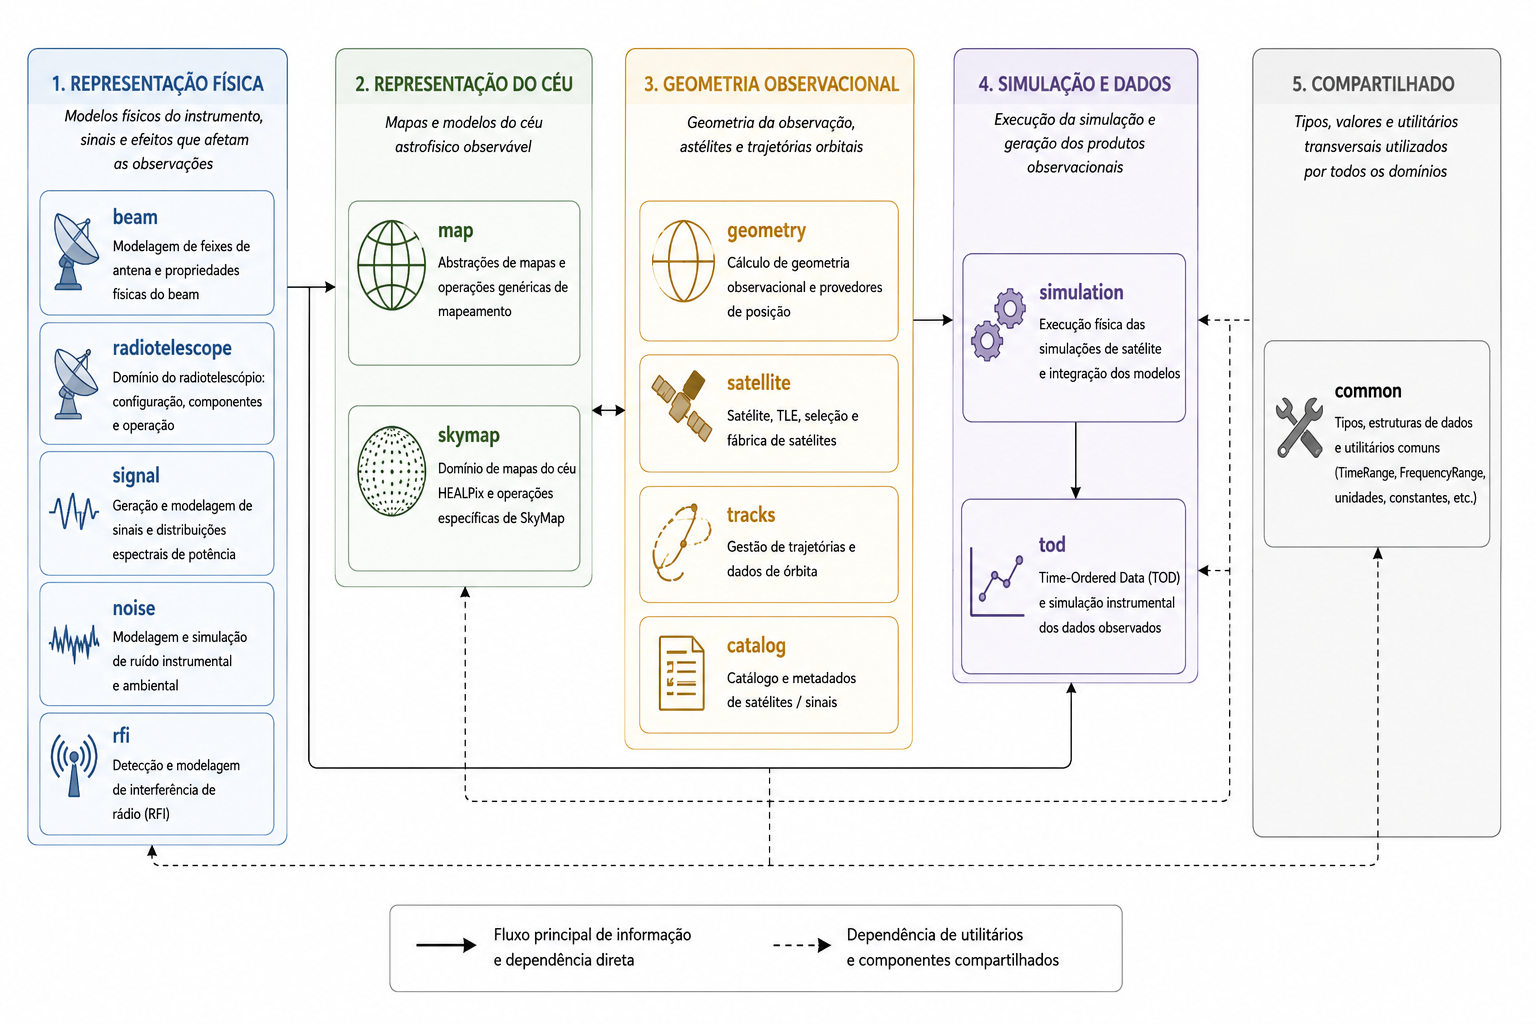
\includegraphics[scale=.32]{Figuras/dominio_pipeline.png}
    \caption{Principais domínios da pipeline de simulação. Fonte: Elaborado pelo autor.}
    \label{fig:diagrama-pipeline-dominios}
\end{figure}

\subsubsection{Domínios de Representação Física}

O domínio de representação física concentra os modelos associados ao instrumento observacional e aos processos físicos que afetam os sinais adquiridos, incluindo a resposta do feixe, a modelagem dos sinais de interesse, os mecanismos de ruído e as fontes de interferência por radiofrequência.. Ele inclui classes como \texttt{beam}, \texttt{radiotelescope}, \texttt{signal}, \texttt{noise} e \texttt{rfi}.

O domínio \texttt{beam} concentra os aspectos relacionados à resposta angular da antena, incluindo parâmetros fisicos e operações aplicadas para modelar o efeito do feixe instrumental sobre os sinais observados. O domínio \texttt{radiotelescope} representa o conjunto de características físicas e operacionais do instrumento de observação, Abrangendo a geometria da antena, a configuração de varredura e os parâmentros de aquisição de dados. 

A modelagem dos sinais observados é realizada por meio do domínio \texttt{signal}, o qual representa os diferentes componentes do sinal, como o sinal astronômico e pela descrição de distribuições espectrais de potência. Complementarmente, o domínio \texttt{noise} tem como missão, modelar os diferentes tipos de ruído presentes nas observações, assim como ruído térmico, ruído de fundo e outras fontes de interferência. O domínio \texttt{rfi} é dedicado à representação de interferências provenientes de fontes artificiais, como satélites e emissões terrestres, permitindo a modelagem de seus efeitos sobre os dados observacionais simulados.

De forma integrada, os dominios de representação física fornecem a base para a construção dos sinais simulados, a aplicação dos efeitos instrumentais e a geração dos dados ordenados no tempo, permitindo que a pipeline produza resultados realistas e cientificamente relevantes para o estudo de fenômenos astronômicos.

\subsubsection{Domínios de Representação do Céu}

A representação do céu observacional é organizada por meio dos domínios \texttt{map} e \texttt{skymap}. Esses módulos são encarregados por armazenar, manipular e processar os mapas de entrada utilizados nas simulações.

O \texttt{map} é focado em definir a estrutura de dados para representação de mapas celestes, abrangendo a definição de atributos como resolução angular, sistema de coordenadas e formato de armazenamento. Por sua vez, o domínio \texttt{skymap} implementa funcionalidades específicas para mapas HEALPix, incluindo mecanismos de acesso aos dados, aplicação de máscaras e manipulação de componentes astrofísicos.
\subsubsection{Domínios Observacionais}

A determinação da geometria observacional e do movimento dos objetos simulados é tratada pelos domínios \texttt{geometry}, \texttt{satellite}, \texttt{tracks} e \texttt{catalog}.

O domínio \texttt{geometry} modela a geometria da observação, como a posição do observador, a orientação do instrumento e a trajetória de varredura. Ele fornece métodos para calcular as coordenadas de observação. O  \texttt{satellite} concentrar as identidades associadas aos satélites artificiais, seus parâmetros orbitais, características de emissão e efeitos de interferência sobre os dados observacionais.

Complementarmente, os domínios \texttt{tracks} e \texttt{catalog} são responsáveis pelo gerenciamento de trajetórias, efemérides e metadados associados aos objetos observados. O domínio \texttt{tracks} assegura o armazenamento e processamento das trajetórias dos objetos simulados, como também, a determinação de suas posições ao longo do tempo e a análise de suas interações com o instrumento de observação. O domínio \texttt{catalog} fornece informações descritivas, classificações, identificadores e demais metadados utilizados durante as simulações.

\subsubsection{Domínios de Simulação e Produtos de Dados}

A execução das simulações e a geração dos produtos observacionais são realizadas pelos domínios \texttt{simulation} e \texttt{tod}.

O domínio \texttt{simulation} atua como elemento central da pipeline, coordenando a execução das diferentes etapas do processo de simulação. Ele fica a cargo de integrar os componentes relacionados à representação física, geometria observacional e manipulação de mapas, garantindo que as simulações sejam conduzidas de forma consistente e alinhada aos requisitos científicos estabelecidos.

Já o domínio \texttt{tod} é encarregado de representar os dados ordenados no tempo produzidos durante as simulações. Ele define a estrutura de dados para armazenar as séries temporais correspondentes às observações simuladas, informações sobre os pontos de amostragem, os valores dos sinais observados e os metadados associados. Esse domínio também implementa métodos para manipular e processar os dados temporais, facilitando a análise e interpretação dos resultados produzidos pela pipeline.

\subsubsection{Domínios Compartilhados}

Por fim, o domínio \texttt{common} reúne os elementos compartilhados entre os diferentes módulos da pipeline, incluindo classes utilitárias, funções de apoio e estruturas de dados comuns. Ele serve como um repositório central para componentes que são utilizados por múltiplos domínios, promovendo a reutilização de código e a consistência em toda a implementação da pipeline. 

A centralização desses componentes reduz redundâncias e contribui para a consistência das interfaces utilizadas pelos diferentes domínios. Essa divisão clara entre domínios especializados e elementos compartilhados favorece a organização do código, facilita a manutenção e promove a evolução independente dos diferentes módulos da pipeline ao longo do tempo. Essa organização constitui a base conceitual da arquitetura implementada e fornece os mecanismos necessários para a construção de cenários observacionais complexos de forma modular e extensível, em consonância com os princípios de modelagem orientada a domínios propostos por \citeonline{evans2003ddd}.

\subsection{Fluxo de Dados}

O fluxo de dados da pipeline foi projetado para integrar informações provenientes de múltiplas fontes e transformá-las em produtos observacionais simulados de forma estruturada e reprodutível. A Figura~\ref{fig:fluxo-dados-pipeline} apresenta uma visão geral desse processo, evidenciando as diferentes camadas da arquitetura e as interações estabelecidas entre seus componentes.

\begin{figure}[hbtp]
    \centering
    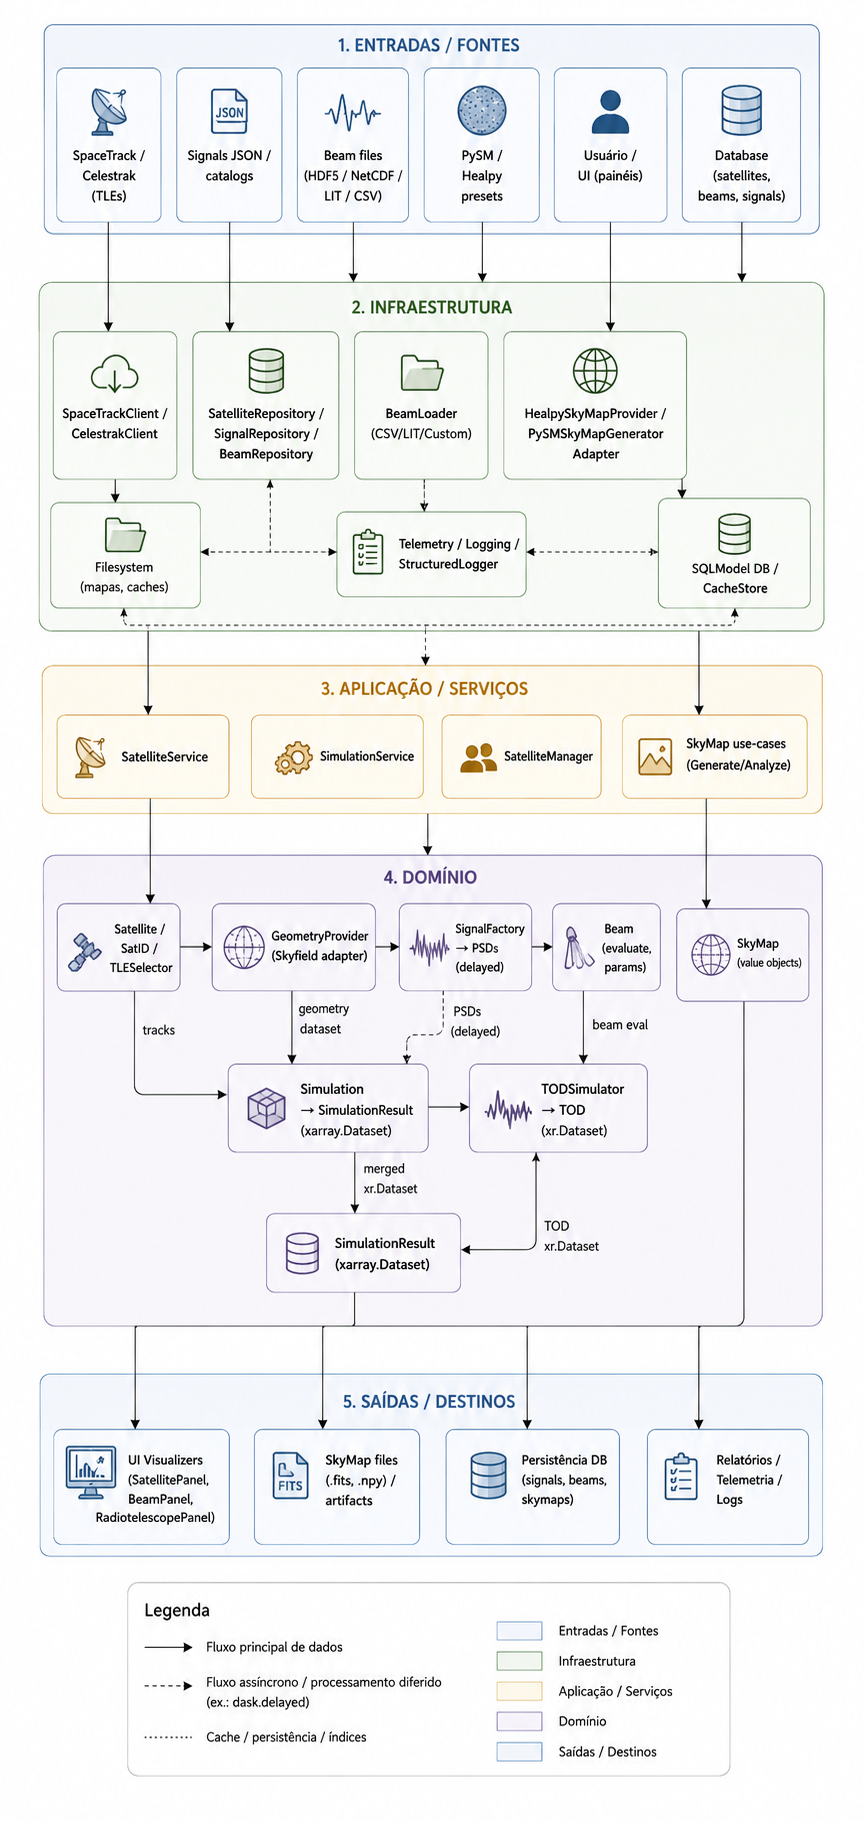
\includegraphics[scale=.38]{Figuras/Fluxo_de_dados.png}
    \caption{Fluxo de dados da pipeline de simulação. Fonte: Elaborado pelo autor.}
    \label{fig:fluxo-dados-pipeline}
\end{figure}

O processo tem início na etapa de aquisição dos dados de entrada, que inclui elementos orbitais de satélites, catálogos de sinais, modelos do feixe instrumental, mapas do céu e parâmetros fornecidos pelo usuário. Esses dados são obtidos por meio de serviços externos, repositórios científicos e interfaces de configuração, sendo processados e organizados para uso nos estagios subsequentes da pipeline.

Após a aquisição, os dados são processados pela camada de infraestrutura, responsavel pela comunicação com serviços externos, gerenciamento de arquivos e persistência das informações. Nessa etapa, os diferentes formatos de entrada são convertidos para representações compatíveis com os modelos utilizados pela pipeline, assegurando a consistência dos dados e propiciando sua manipulação nos processos seguintes. Além disso, mecanismos de armazenamento temporário e cache são empregados para otimizar o acesso aos dados e reduzir a latência durante a execução das simulações.

A camada de aplicação atua como intermediária entre os componentes de infraestrutura e os modelos científicos do domínio. Seus serviços coordenam operações relacionadas à obtenção de satélites, geração de mapas do céu e execução das simulações, encapsulando regras de negócio e certificando a integridade dos processos. Essa camada é responsável por orquestrar as interações entre os diferentes módulos, assegurando que as etapas de processamento sejam conduzidas de forma consistente e alinhada aos requisitos científicos estabelecidos para o projeto.

No núcleo da arquitetura encontram-se os modelos científicos responsáveis pela representação dos satélites, da geometria observacional, dos sinais simulados, dos mapas do céu e da resposta instrumental.  Nessa etapa, os elementos orbitais são convertidos em trajetórias observacionais, os modelos geométricos determinam a posição relativa entre o instrumento e os objetos simulados, e os sinais são gerados a partir dos modelos físicos definidos para cada cenário. Essas informações são então combinadas para produzir os dados observacionais sintéticos.

O domínio de simulação coordena a aplicação dos efeitos instrumentais sobre os sinais gerados, levando em consideração a geometria da observação e as características do feixe. O resultado desse processo é a produção dos dados ordenados no tempo (\textit{Time Ordered Data} -- TOD), que representam as séries temporais correspondentes às observações simuladas.

Os produtos gerados pela pipeline podem ser direcionados para diferentes destinos. Entre eles destacam-se as interfaces de visualização, os arquivos científicos utilizados em análises posteriores, os bancos de dados destinados à persistência dos resultados e os sistemas de telemetria empregados para monitoramento e rastreabilidade das execuções. Essa flexibilidade permite que os mesmos dados sejam utilizados em diferentes etapas do ciclo de desenvolvimento, validação e análise científica.

Além disso, a organização adotada estabelece uma separação clara entre aquisição de dados, processamento científico e geração de produtos observacionais. Essa estrutura reduz o acoplamento entre os componentes da arquitetura e permite a evolução independente dos diferentes módulos da pipeline. Como resultado, novas fontes de dados, modelos físicos e estratégias de simulação podem ser incorporados sem alterações significativas nos demais componentes do sistema, preservando a consistência da implementação e a reprodutibilidade dos experimentos realizados \cite{evans2003ddd, martin2008cleancode}.

\section{Casos de Uso}
 
Nesta seção, são apresentados casos de uso exemplares que ilustram a aplicação da pipeline de simulação em cenários específicos de interesse científico. Cada caso de uso descreve o contexto, os objetivos, os passos envolvidos na execução da simulação e os resultados esperados, demonstrando a flexibilidade e a capacidade da pipeline para atender a diferentes necessidades de pesquisa em radioastronomia observacional.

\subsection{Geração de Mapas do Céu Sintéticos}

A geração de mapas do céu sintéticos é um caso de uso fundamental da pipeline, uma vez que  que fornece a representação espacial dos sinais astronômicos simulados, servindo como base para a construção dos dados observacionais \cite{delabrouille2013psm, thorne2017pysm}. Esses mapas descrevem a distribuição da intensidade do sinal celeste sobre a esfera celeste, discretizada segundo a pixelização HEALPix \cite{gorski2005healpix}, permitindo sua utilização em estudos de observação simulada, reconstrução de mapas e análise de efeitos instrumentais.

Para atender a essa necessidade, foi desenvolvido o caso de uso \texttt{GenerateSkyMapUseCase}, responsável por coordenar o processo de criação de mapas sintéticos a partir dos parâmetros definidos. Sua implementação está localizada na camada de aplicação da arquitetura e segue os princípios de separação de responsabilidades adotados ao longo do projeto.

O processo de geração de mapas inicia-se com a definição dos parâmetros de entrada, que incluem parâmetro $N_{\mathrm{side}}$, a frequência de observação e a lista de componentes físicos que devem compor o sinal simulado. Esses parâmetros são fornecidos por meio de uma interface de configuração, permitindo que o usuário personalize a simulação de acordo com suas necessidades específicas. O parâmetro $N_{\mathrm{side}}$ determina a resolução angular do mapa HEALPix, enquanto a frequência de observação influencia a modelagem dos sinais astronômicos e dos efeitos instrumentais.

Antes de iniciar a criação do mapa, o caso de uso realiza uma validação dos parâmetros de entrada, assegurando que estejam dentro dos limites aceitáveis e que sejam consistentes com os modelos físicos disponiveis na pipeline. A frequência de observação deve assumir valores positivos e ao menos um componente físico deve ser especificado para a construção do mapa. Caso os parâmetros sejam considerados inválidos, o processo é interrompido e uma mensagem de erro é retornada ao usuário, indicando a natureza da inconsistência detectada.

Após a validação, o caso de uso converte o valor informado para um objeto de domínio do tipo \texttt{NSide}, que encapsula propriedades relacionadas à resolução angular do mapa HEALPix. Em seguida, a geração do mapa é delegada à interface \texttt{SkyMapGeneratorPort}, que define o contrato utilizado para comunicação entre a camada de aplicação e os mecanismos concretos de geração implementados na infraestrutura.

Como resultado, é produzido um objeto contendo os dados do mapa gerado, o número total de pixels e a resolução utilizada. Essas informações são encapsuladas em um objeto de transferência de dados (\textit{Data Transfer Object} -- DTO) \cite{evans2003ddd}, permitindo que os resultados sejam consumidos por outros componentes da pipeline sem dependência direta das implementações internas do processo de geração.

O Código~\ref{lst:generate-skymap} apresenta uma versão simplificada do fluxo de execução do caso de uso.

\begin{lstlisting}[
language=Python,
caption={Trecho simplificado do caso de uso de geração de mapas sintéticos.},
label={lst:generate-skymap}
]
def execute(input_dto):

    nside = NSide(input_dto.nside)

    sky_map = generator.generate(
        nside=nside,
        freq_ghz=input_dto.frequency_ghz,
        components=input_dto.components,
    )

    return GenerateSkyMapOutputDTO(
        nside=nside.value,
        npix=sky_map.npix,
        map_data=sky_map.data,
    )
\end{lstlisting}

A separação entre validação, coordenação da execução e geração física do mapa permite que diferentes mecanismos de construção de mapas sejam incorporados à pipeline sem alterações na lógica de aplicação. Dessa forma, novos modelos astrofísicos ou bibliotecas especializadas podem ser integrados por meio da implementação da interface \texttt{SkyMapGeneratorPort}, preservando a estabilidade da arquitetura e favorecendo sua extensibilidade.

\subsection{Análise de Mapas do Céu}

Após a aquisição de mapas do céu, é necessário realizar análises para extrair informações quantitativas sobre os sinais simulados. Geralmente, em estudos radioastronômicos, uma abordagem amplamente utilizada consiste na decomposição do mapa em harmônicos esféricos e na análise do espectro de potência angular associado \cite{gorski2005healpix}. O espectro angular $(C_\ell)$ fornece uma medida da distribuição de potência em diferentes escalas angulares do sinal observado, constituindo uma ferramenta fundamental para caracterização de estruturas presentes nos mapas celestes.

Com esse objetivo, a pipeline implementa o caso de uso \texttt{AnalyzeSkyMapUseCase}, responsável por coordenar a análise espectral de mapas representados pelo objeto de domínio \texttt{SkyMap}. Sua implementação segue a mesma filosofia arquitetural adotada nos demais casos de uso defendida por Evans \cite{evans2003ddd} e Martin \cite{martin2008cleancode}, concentrando-se na validação dos parâmetros de entrada e na orquestração da execução da análise.

A execução se inicia com o recebimento de um objeto contendo o mapa a ser analisado e, opcionalmente, o valor máximo do multipolo angular $(\ell_{\mathrm{max}})$. A priori, são realizadas verificações para assegurar que o mapa fornecido seja válido e compativel com a estruttura de dados utilizada pela pipeline. O mapa deve conter um número de pixels consistente com a resolução angular definida pelo parâmetro $N_{\mathrm{side}}$, e os dados devem estar organizados de acordo com o formato HEALPix.

Em seguida, o caso de uso delega o calculo do espectro de potência angular à interface \texttt{SkyMapAnalyzerPort}, que define o contrato para comunicação entre a camada de aplicação e os mecanismos concretos de análise implementados na infraestrutura. O resultado desse processo é um objeto contendo os valores do espectro de potência angular para cada multipolo até o valor máximo especificado. Esses resultados são encapsulados em um DTO, permitindo que sejam consumidos por outros componentes da pipeline para análises posteriores ou visualização.

O Código~\ref{lst} apresenta um trecho simplificado da execução desse caso de uso.

\begin{lstlisting}[
language=Python,
caption={Trecho simplificado do caso de uso de análise de mapas do céu.},
label={lst}
]
cls = self._analyzer.compute_cls(
skymap=sky_map,
lmax=input_dto.lmax,
)

return AnalyzeSkyMapOutputDTO(
nside=sky_map.nside_value,
lmax=input_dto.lmax,
cls=cls,
)
\end{lstlisting}

Observa-se que a separação entre validação, coordenação da execução e análise física do mapa permite que diferentes algoritmos de análise sejam incorporados à pipeline sem alterações na lógica de aplicação. Além disso, esse caso de uso pode ser empregado na análise de mapas provenientes de observações reais ou de outras ferramentas de simulação.



\section{Estrutura do Código}

A implementação da pipeline de simulação foi organizada em uma estrutura de código modular, seguindo os princípios de engenharia de software e as melhores práticas de desenvolvimento. A estrutura adotada reflete a arquitetura definida para o sistema, facilitando a manutenção, evolução e colaboração entre os desenvolvedores.

\subsection{Organização de Diretórios}

A organização do código-fonte foi concebida para refletir diretamente a arquitetura apresentada nas seções anteriores, adotando princípios de separação de responsabilidades, baixo acoplamento e independência entre domínios científicos e componentes tecnológicos. A estrutura do projeto segue uma divisão em camadas, permitindo que os modelos científicos permaneçam desacoplados dos mecanismos de persistência, interfaces de usuário e bibliotecas externas. A estrutura de diretórios é organizada da seguinte forma: 

A Figura~\ref{fig:estrutura-codigo} apresenta uma visão resumida da organização dos principais diretórios do projeto.

\begin{figure}[hbtp]
    \centering
    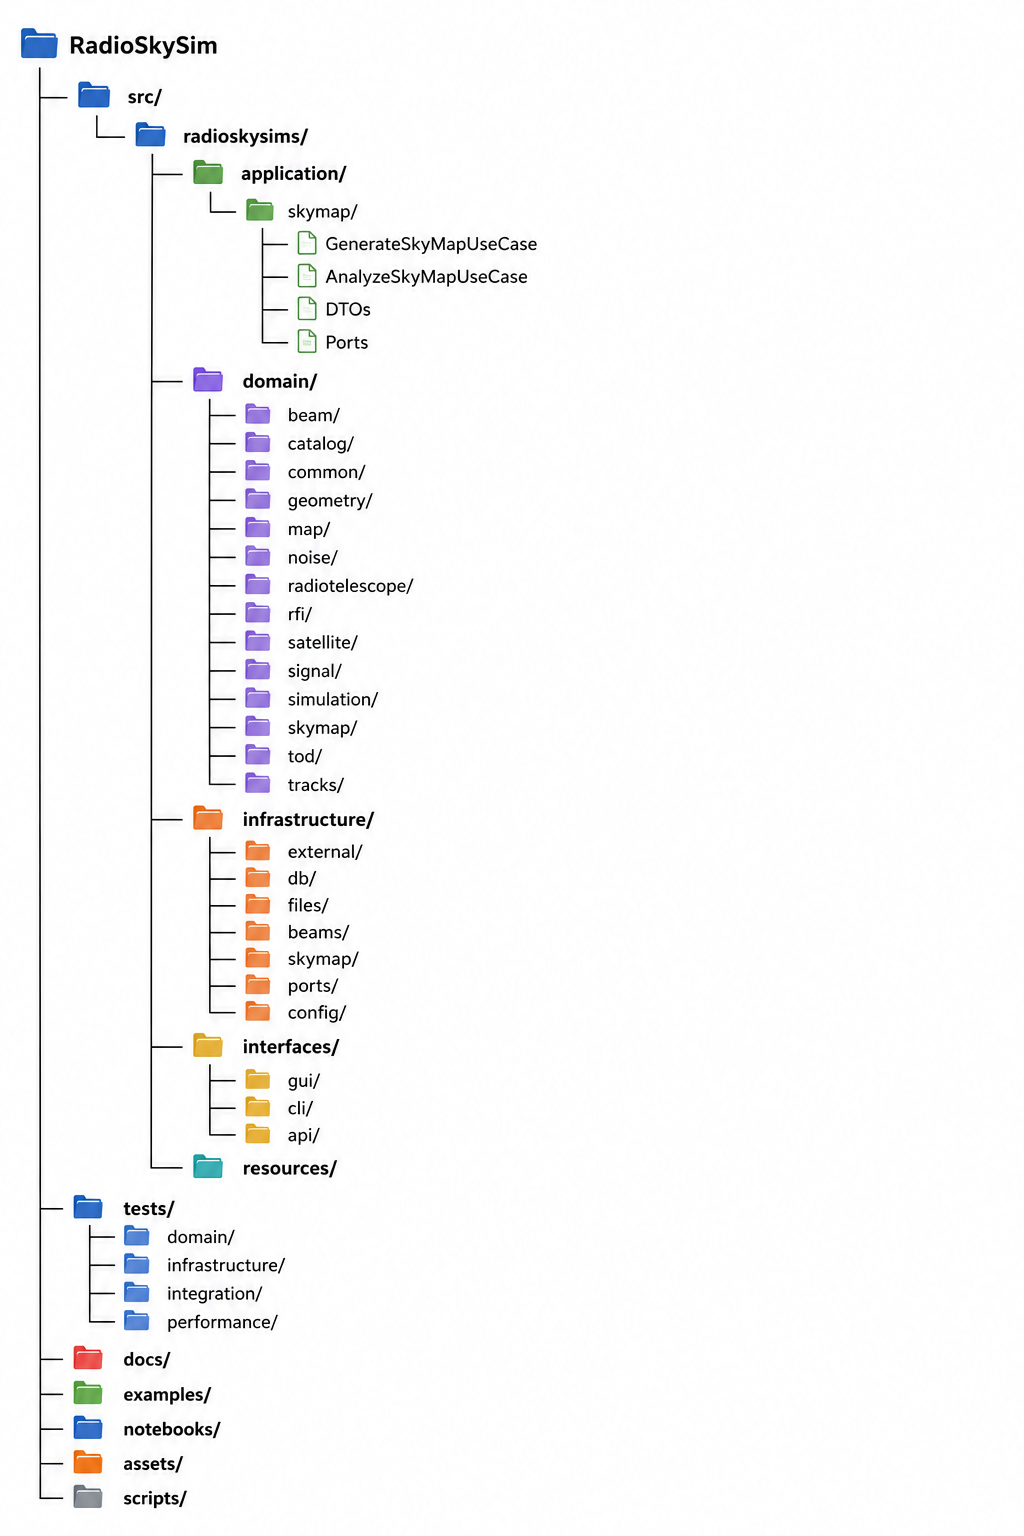
\includegraphics[scale=.4]{Figuras/Organização_diretorio.png}
    \caption{Estrutura de diretórios do código-fonte da pipeline de simulação. Fonte: Elaborado pelo autor.}
    \label{fig:estrutura-codigo}
\end{figure}

Os componentes centrais da aplicação estão localizados no diretório \texttt{src/radioskysims}, que concentra a implementação da pipeline científica. Sua organização segue uma divisão em quatro grupos principais: aplicação, domínio, infraestrutura e interfaces.

O diretório \texttt{domain} reúne os modelos científicos e conceitos fundamentais utilizados pela pipeline. Nessa camada encontram-se os domínios responsáveis pela modelagem do céu, instrumentação, sinais, ruídos, satélites, geometria observacional e dados ordenados no tempo. A organização interna desse diretório reflete a divisão em domínios apresentada na seção de modelagem \ref{sec.modelagem}, permitindo que cada módulo seja desenvolvido e mantido de forma independente, favorecendo a evolução científica da pipeline ao longo do tempo.

A camada de aplicação, localizada no diretório \texttt{application}. Tem como missão coordenar a execução dos casos de uso, realizar validações de entrada e orquestrar as interações entre os diferentes domínios científicos e os mecanismos de infraestrutura. Os casos de uso de geração e análise de mapas do céu apresentados anteriormente são exemplos de funcionalidades implementadas nessa camada.

Os componentes responsáveis pela comunicação com sistemas externos encontram-se no diretório \texttt{infrastructure}, que inclui implementações de repositórios, adaptadores para serviços externos, mecanismos de persistência, carregamento de arquivos científicos e implementações concretas das portas utilizadas pela aplicação.

As interfaces que é disponibilizadas para interação com o usuário são organizadas no diretório \texttt{interfaces}. Nesse modulo estão incluido  aplicações gráficas, interfaces de linha de comando e possíveis serviços de API.

Complementando a estrutura principal, o diretório \texttt{tests} reúne testes unitários, testes de integração e avaliações de desempenho. Essa organização favorece a validação sistemática dos componentes implementados e contribui para a confiabilidade dos resultados produzidos pela pipeline.

\subsection{Módulos Principais}

A implementação da pipeline foi organizada em módulos especializados, cada um responsável por uma parcela específica da modelagem científica. Os módulos principais da aplicação correspondem aos elementos fundamentais envolvidos na geração dos dados observacionais simulados, abrangendo desde a representação do céu até a produção dos dados ordenados no tempo e dos produtos finais da simulação.


\subsubsection{Módulo SkyMap}

O módulo \texttt{skymap} é responsável pela representação dos mapas do céu utilizados pela pipeline. Sua implementação baseia-se na pixelização HEALPix, amplamente empregada em aplicações astronômicas devido à sua capacidade de representar dados sobre a esfera com resolução uniforme \cite{gorski2005healpix}.

Além do armazenamento dos mapas, esse módulo fornece operações para leitura, escrita, mascaramento, transformação e análise de dados observacionais. Os objetos definidos nesse domínio constituem a principal interface entre os modelos astrofísicos de entrada e os processos de simulação observacional.

\subsubsection{Módulo Beam}

O \texttt{beam} concentra a modelagem da resposta angular do instrumento. Ele define estruturas responsáveis por representar padrões de feixe, parâmetros instrumentais e métodos de avaliação da resposta da antena em diferentes direções do céu.

A modelagem do feixe desempenha papel fundamental na simulação observacional, pois determina como a distribuição de brilho celeste é convoluída pela resposta espacial do instrumento durante o processo de aquisição dos dados.

\subsubsection{Módulo Satellite}

 A representação dos satélites artificiais considerados nas simulações fica a cargo do \texttt{satellite}. Ele reúne entidades associadas aos elementos orbitais, identificadores NORAD, seleção de satélites e construção de cenários observacionais envolvendo diferentes constelações.

Esse módulo atua em conjunto com os componentes de geometria observacional para determinar a posição aparente dos satélites ao longo do tempo e avaliar sua contribuição para os sinais simulados.

\subsubsection{Módulo Geometry}

O \texttt{geometry} implementa os cálculos necessários para determinar a geometria observacional entre o radiotelescópio e os objetos simulados. Suas funcionalidades incluem o cálculo de azimute, elevação, distância e demais parâmetros geométricos utilizados durante a geração dos sinais observacionais.

Os resultados produzidos por esse módulo servem como entrada para os processos de modelagem instrumental e geração dos dados ordenados no tempo.

\subsubsection{Módulo Signal}

Quem se encarregar pela modelagem dos sinais eletromagnéticos que são considerados na simulação é o \texttt{signal}. Ele define mecanismos para geração de distribuições espectrais de potência, modelagem de emissões provenientes de satélites e construção dos sinais utilizados durante a geração dos dados sintéticos.

Sua arquitetura permite a incorporação de diferentes modelos espectrais, favorecendo a extensibilidade da pipeline para novos cenários científicos.

\subsubsection{Módulo TOD}

O \texttt{tod} implementa a geração e manipulação dos dados ordenados no tempo (\textit{Time Ordered Data} -- TOD). Esses dados representam a forma mais próxima das observações produzidas pelo instrumento antes das etapas de reconstrução de mapas.

Nesse módulo são aplicados os efeitos instrumentais, a geometria observacional e os sinais simulados, resultando em séries temporais que reproduzem o processo de aquisição dos dados pelo radiotelescópio.

\subsubsection{Módulo Simulation}

O módulo \texttt{simulation} atua como elemento central da pipeline. Sua função consiste em coordenar a interação entre os diferentes módulos científicos, integrando informações provenientes da geometria observacional, dos modelos de sinal, dos feixes instrumentais e dos dados orbitais.

Ao final da execução, ele produz objetos de resultado que consolidam os produtos gerados durante a simulação, incluindo dados temporais, parâmetros observacionais e informações auxiliares necessárias para análises posteriores.
